\begin{figure}[H]
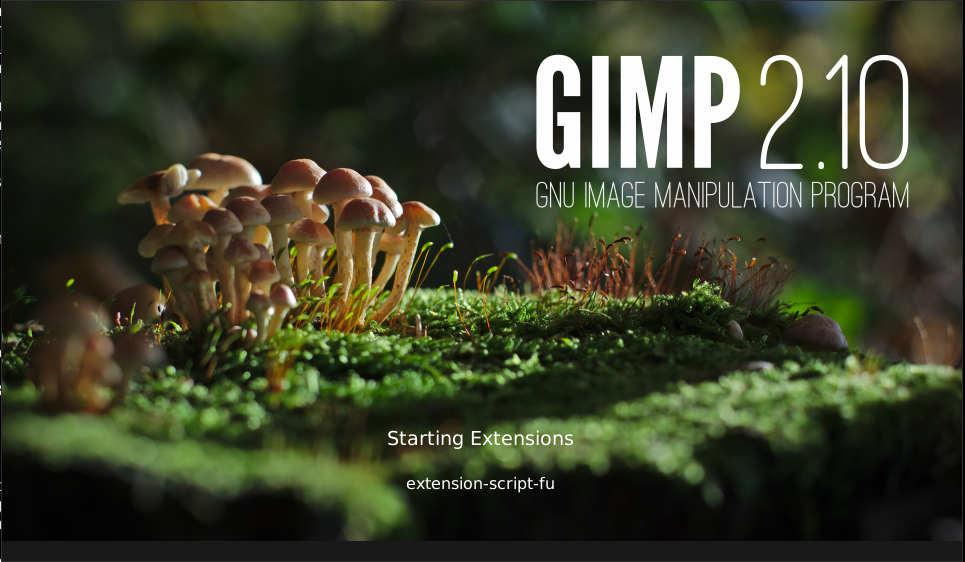
\includegraphics[width=\linewidth]{Gimp-splash.png}
\end{figure}

De GIMP is een applicatie om foto's te bewerken. Je kan het vergelijken met Photoshop van Adobe. Voor diegene die gewend zijn om te werken met Photoshop zal de interface aan de ene kant bekend voorkomen en aan de andere kant net even anders zijn.

\begin{figure}[H]
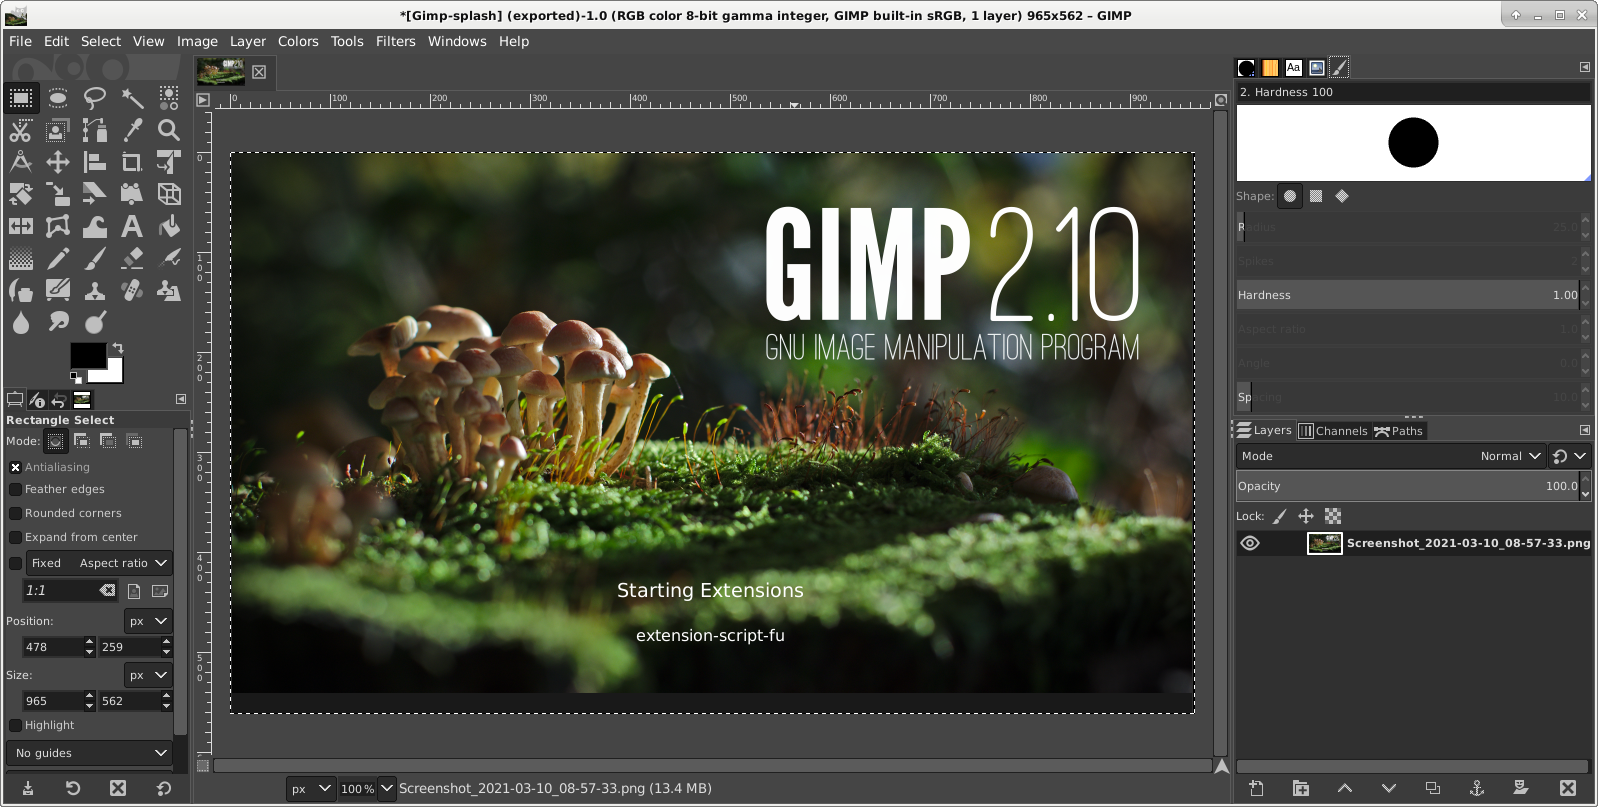
\includegraphics[width=\linewidth]{Gimp-work.png}
\end{figure}
